\chapter{A complete methodology for the implementation of XFEM inclusive models}
\label{sec:a_complete_methodology_for_the_implementation_of_XFEM_inclusive_models}

% -----------------------------------------------------------------------------
% Abstract.

This document was written in 2012 as an internal implementation manual for future developers of our code, the Finite Element Multi-Disciplinary Optimization Code (femdoc).

This report offers a background into the eXtended Finite Element Method as a tool to solve the shortcomings of the classical Finite Element Method. An example of such is the numerical solution to problems with different material topologies (i.e. discontinuities). The XFEM uses level set functions to track the location of these discontinuities. The report also provides algorithms for locating these discontinuities and subsequently dividing the domain into sub-domains capable of integration. This report ultimately expounds upon how to effectively apply the local enrichment functions that the XFEM standard approximation requires at the nodes where the discontinuities occur.

The reader may skip this section, as it focuses on the algorithmic implementation of the framework and most of its content is intended for software developers.

% -----------------------------------------------------------------------------
% Chapters.

% XFEM: Background.
\section{Introduction}
\label{introduction}

% -----------------------------------------------------------------------------
% Finite element method.

\subsection{Finite element method}

The Finite Element Method (FEM) is a numerical technique used for finding solutions to partial differential equations as well as to integral equations. Traditional finite element methods (FEM) requires meshing techniques that generate discrete representation of potentially complex geometry. Difficulties arise when using the traditional FEM for analyzing fracture mechanics: under traditional FEM, introducing a discontinuity in the mesh, changing the material topology or drastically changing the shape of the material requires a new mesh to ensure that the element edges align with the discontinuity \citep{AH:08}. The process is laborious and difficult \citep{ZTZ:05}. The eXtended Finite Element Method (XFEM) arose as a solution to this impediment by applying enrichment functions at the position of the material interface or topology discontinuity instead of re-meshing the entire structure.

% -----------------------------------------------------------------------------
% Discontinuity

\subsection{Discontinuity}

A discontinuity can be defined as a rapid change in a field variable over a length negligible in size compared to the entire domain analyzed \citep{AH:08}. For example, in solid mechanics, strain and stress fields are discontinuous across material interfaces and displacements are discontinuous at cracks; in fluid dynamics, velocity and pressure fields are discontinuous at the boundary layer between two fluids. A discontinuity is classified as ``weak'' or ``strong''. Weak discontinuities happen when a field variable (stress field, strain rate, etc.) has a kink, meaning the derivative has a jump. This can happen at boundary layers, or at a material or fluid interface. Strong discontinuities happen when the field quantity has a jump; this could include, for example, a crack in the structure \citep{HH:04b}.

%----------------------------------------------------------------------------------------
% eXtended Finite Element Method

\subsection{eXtended Finite Element Method}

The XFEM arose as a numerical technique capable of providing local enrichment functions at the position of the material interface, avoiding the need to re-mesh the entire structure while finding solutions for the discontinuous functions \citep{FB:10}. By doing this, XFEM appears to solve the shortcomings of the FEM by providing accurate solutions for complex problems in engineering that would be impossible to solve otherwise \citep{AH:08}.

%----------------------------------------------------------------------------------------
% Level set method

\subsection{Level set method}

Level set functions are used to model the motion of these discontinuities in the elements. A level set function is a numerical scheme where the discontinuity of interest is represented as the zero level set function. Basically, a level set function has a value of zero at the boundary of its closed curve and opposite signs on the interior and the exterior (Figure \ref{fig:Level-Set}).
%
\begin{equation}
	\centering
	\begin{split}
		\phi\left(\mathbf{x}\right) > 0 & \quad \forall \mathbf{x} \in \Omega \backslash \partial \Omega \text{ (inside the region)} \\
		\phi\left(\mathbf{x}\right) = 0 & \quad \forall \mathbf{x} \in \partial \Omega \text{ (on the boundary)} \\
		\phi\left(\mathbf{x}\right) < 0 & \quad \forall \mathbf{x} \in D \backslash \Omega \text{ (outside the region)}
	\end{split}
\end{equation}
%
The XFEM uses this method by placing the discontinuity at the boundary layer and giving the interface caused by the division positive and negative values. Since the zero level is interpreted as the discontinuity, new nodes (called pseudo-nodes) are created at this position and the enrichment of the FEM is produced at this location. This creates an advantage because instead of re-meshing the entire structure, a fixed Cartesian grid is used to divide the structure and the discontinuity into domains capable of integration. Once this mesh is settled, the XFEM will subsequently use either branched or Heaviside functions to enrich the nodes and solve for the problem.
%
\begin{figure}[H]
	\centering
	\begin{tabularx}{\linewidth}{XX}
		\subfloat[]{
			\label{fig:level_set_circle_func_impl_1}
			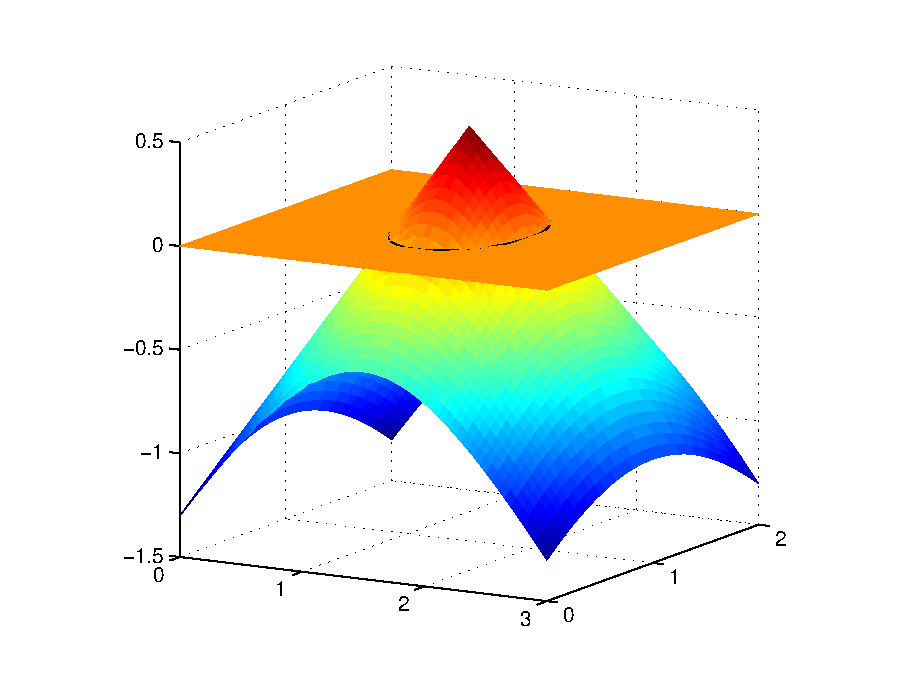
\includegraphics[width=\linewidth]{level_set_circle_func_050.eps}
		} &
		\subfloat[]{
			\label{fig:level_set_circle_domain_impl_1}
			\includegraphics[width=\linewidth]{level_set_circle_domain_050.eps}
		}
	\end{tabularx}
	\caption{The zero level set isolevel of the level set function, $\partial \Omega = \Gamma_{\phi=0}$, in \ref{fig:level_set_circle_func_impl_1} divides the fixed mesh grid into different phase regions in \ref{fig:level_set_circle_domain_impl_1}, where each phase may represent a different material or a different physics.}
	\label{fig:Level-Set}
\end{figure}

The Level Set Method (LSM) and the XFEM have a sort of natural coupling to solve problems with discontinuities. While the LSM is used to model the discontinuity and update its motion at each calculation, the XFEM is used to solve the problem and determine the direction of the discontinuity \citep{SCM+:01}.

% -----------------------------------------------------------------------------
% Delaunay triangulation

\subsection{Delaunay triangulation}

In order to apply the LSM and the XFEM to solve a problem, a framework for dividing arbitrarily complex geometries into integrable domains must be developed. The Delaunay triangulation is a critical step in this process. The Delaunay triangulation is the subdivision of a geometric object into triangles for 2D geometry and tetrahedra for 3D (Figure \ref{fig:Delaunay-Triangulation}). This particular triangulation has the property that the circumcircle of any triangle in the triangulation does not contain the vertices of other triangles or its own in its interior (Figure \ref{fig:Delaunay-Circumcircles}) \citep{LS:80}. Because triangle and tetrahedra are integrable elements, the XFEM method can then be applied.

\begin{figure}[htbp]
	\centering
		\includegraphics[width=0.75\linewidth]{delaunay_triangulation.eps}
	\caption[Delaunay triangulation]{The Delaunay formulation triangulates QUAD4 finite elements cut by the level set zero isolevel from Figure \ref{fig:level_set_circle_domain_impl_1} into TRI3 elements.}
	\label{fig:Delaunay-Triangulation}
\end{figure}

\begin{figure}[htbp]
	\centering
	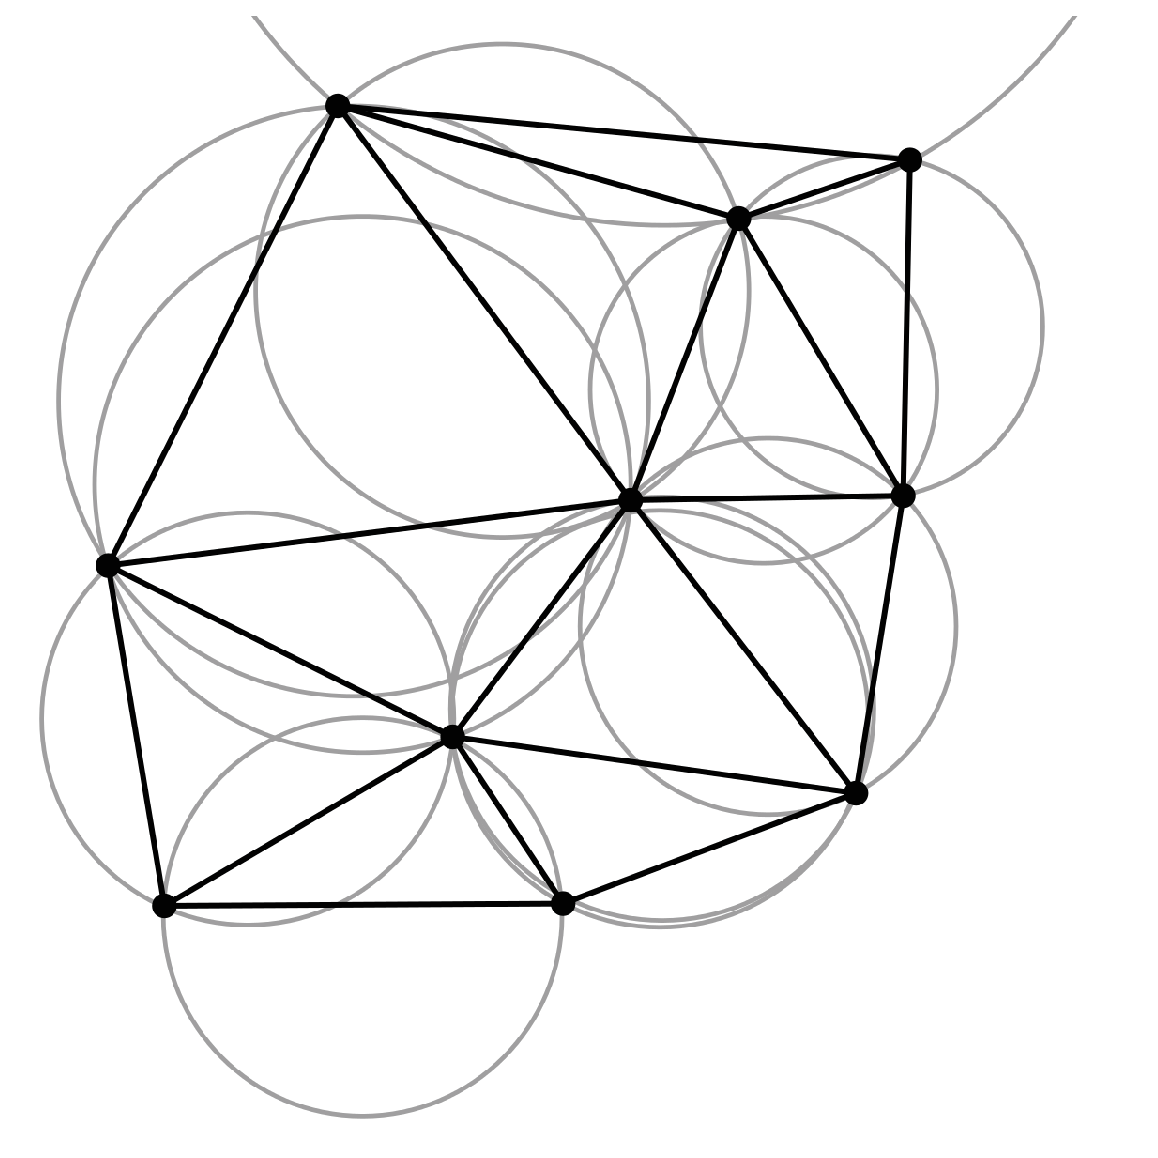
\includegraphics[width=0.5\linewidth]{delaunay_circumcircles.eps}
	\caption[Delaunay circumcircles]{Delaunay circumcircles - A set of points can be uniquely triangulated in a way that the points form circumcircles.}
	\label{fig:Delaunay-Circumcircles}
\end{figure}

For an inclusion-based XFEM model (inclusion meaning the zero level function is always a closed curve), there are only 8 triangulation configurations in 2D, while 127 different ones in 3D. Due to the low number of cases in 2D, a tabulation of the triangulation is performed instead of using the Delaunay triangulation. Figure \ref{fig:intersections_2D} shows the different cases for 2D, while Figure \ref{fig:intersections_3D} shows the triangulation of a 3D element with four different discontinuities.

\begin{figure}[htbp]
	\centering
		\includegraphics[width=\linewidth]{intersections_2D.eps}
	\caption[2D triangulation configurations]{There are only 8 different triangulation configurations for an inclusion-based XFEM model.}
	\label{fig:intersections_2D}
\end{figure}

\begin{figure}
	\centering
	\begin{tabularx}{\linewidth}{XXX}
		\subfloat[Phase ``A''.]{
			\label{fig:intersections_3D_1}
			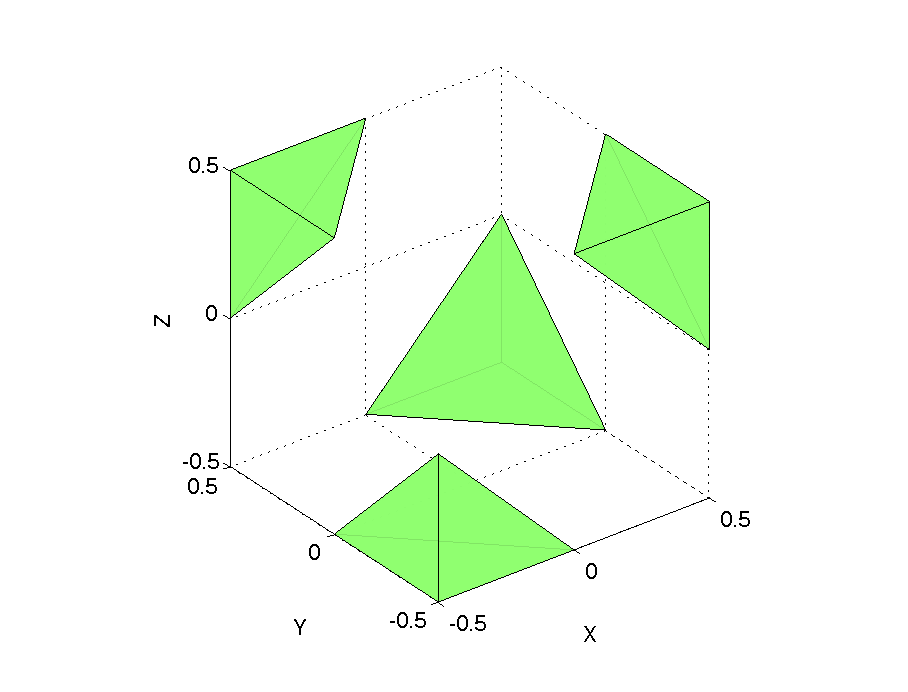
\includegraphics[width=\linewidth]{intersections_3D_1.eps}
		} &
		\subfloat[Phase ``B''.]{
			\label{fig:intersections_3D_2}
			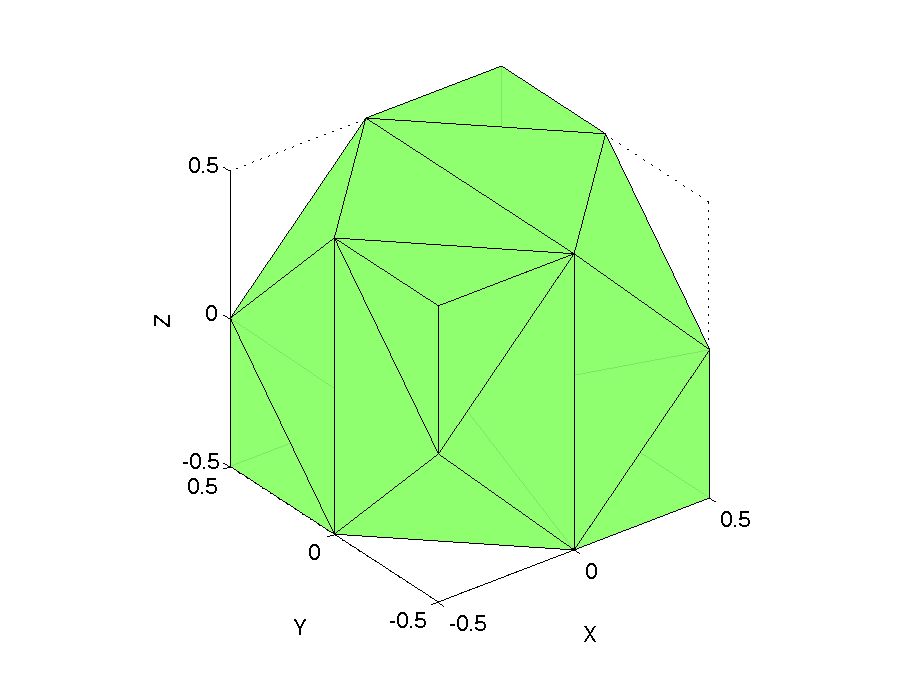
\includegraphics[width=\linewidth]{intersections_3D_2.eps}
		} &
		\subfloat[Both phase regions.]{
			\label{fig:intersections_3D_3}
			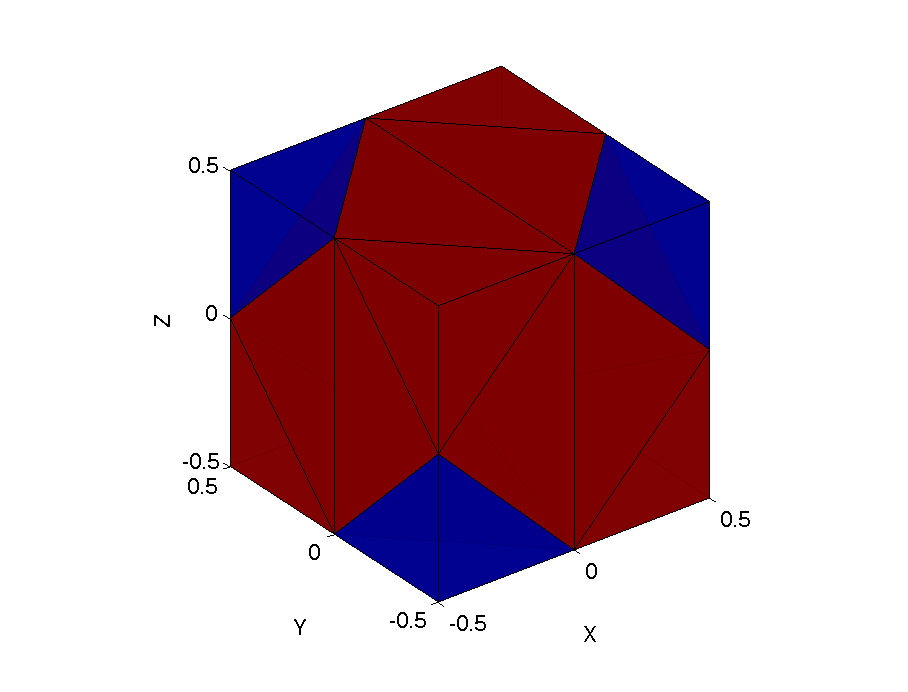
\includegraphics[width=\linewidth]{intersections_3D_3.eps}
		}
	\end{tabularx}
	\caption[3D triangulation example.]{Triangulation in 3D is more complex and we use the Delaunay triangulation algorithm to perform the computation. This element with 4 discontinuities has 4 pseudo-elements from material phase 1 and 20 from material phase 2.}
	\label{fig:intersections_3D}
\end{figure}
\section{Implementation}
\label{implementation}

%----------------------------------------------------------------------------------------
% Summary

\subsection{Summary}

This document outlines the procedure for building an XFEM model for a given distribution of the level-set function. The XFEM model consists of:
\begin{itemize}
\item Intersection points along elemental edges.
\item XFEM elements sub-divided into cells for integrating the weak form of the governing equations within the individual sub-domains belonging to a particular material phase.
\item Enrichment tables that define the nodal enriched degrees of freedom used to interpolate the solution within a cell.
\item Parallel implementation of building XFEM model.
\end{itemize}

%----------------------------------------------------------------------------------------
% Glossary

\subsection{Glossary}

\noindent
\textbf{computational mesh} -- standard FE mesh that defines the nodal degrees of freedom. \\
\textbf{model} -- physical entity, contains information about the XFEM elements and the level-set functions. \\
\textbf{main phase (phase)} -- phase indicating a particular material phase. \\
\textbf{sub-phase} -- the domain of a main phase can be decomposed into multiple sub-phases. \\
\textbf{intersection point} -- intersection created by the zero level-set curve cutting through an edge. \\
\textbf{point} -- geometrical entity with information about coordinates, connected cells and edges. \\
\textbf{cell} -- geometrical entity, a collection of points, owns a list of edges too. \\
\textbf{edge} -- geometrical entity with information about the points on its ends and its connected cells. \\
\textbf{Delaunay triangulation} -- triangulation of our elements using their corner nodes and intersection points. \\
\textbf{pseudo-element} -- cells created by the triangulation of the regular element. \\
\textbf{nodal cluster} -- set of elements (and their nodes) connected to a node
consistency nodes	nodes shared by multiple elements within nodal cluster. \\

%----------------------------------------------------------------------------------------
% Procedure

\subsection{Procedure overview}

The main steps are:
\begin{enumerate}
\item Build point-to-cells connectivity list (list of cells connected to a point) by looping over all cells; needs to be built only once.
\item Build edge table in mesh (list of the cell edges that stores connectivity to points and cells) by looping over all cells; needs to be built only once.
\item Build table of nodes belonging to a nodal cluster (first-order neighbors of a node; defined as all nodes belonging to elements connected to a node) by looping over all elements for a node using point-to-cell table; needs to be built only once.
\item Build edge intersection points by looping over all edges; points are stored in mesh; however, the coordinates of the intersections are copied to the XFEM element; needs to be built for each instance of a level-set distribution.
\item Delaunay triangulation of each cell based on edge intersection; needs to be built for each instance of a level-set distribution.
\item Build table of phases and sub-phases for each triangle/tetrahedron (pseudo-cells) for each triangulated element; needs to be performed for each instance of level set distribution.
\item Build enrichment table that defines which nodal degrees of freedom are used to interpolate a field within a pseudo-element.
\item Determine which degrees of freedom are used in the model.
\end{enumerate}

%\begin{figure}[htbp]
%	\centering
%	\includegraphics[scale=1]{./img/procedure_overview.png}
%	\caption[XFEM Overall Procedure]{The diagram shows the overall procedure required to implement the XFEM model.}
%	\label{fig:Overall-Procedure}
%\end{figure}

% -----------------------------------------------------------------------------
% XFEM implementation algorithms

\subsection{Implementation algorithms}
\label{sec:implementation}

Consider the following XFEM model which consists of a 4-element mesh in 2D; the nodes on the left are clamped and the right edge is subject to a constant pressure load. The level-set distribution in Figure \ref{fig:structural_model} leads to the intersection pattern shown in Figure \ref{fig:physical_model}. The mesh in Figure \ref{fig:discrete_model} shows the indices of the nodes and the cells.

\begin{figure}[htbp]
	\centering
	\includegraphics[width=0.75\linewidth]{structural_model.eps}
	\caption[Structural problem setup.]{Structural problem setup. The domain contains multiple level set inclusions.}
	\label{fig:structural_model}
\end{figure}

\begin{figure}[htbp]
	\centering
	\includegraphics[width=0.75\linewidth]{physical_model.eps}
	\caption[XFEM implementation example physical model]{4-element 2D mesh. Black areas: material phase 1, negative level-set value at the nodes; white areas: material phase 2, positive level-set value.}
	\label{fig:physical_model}
\end{figure}

\begin{figure}[htbp]
	\centering
	\includegraphics[width=0.75\linewidth]{discrete_model.eps}
	\caption[XFEM implementation example discrete model]{4-element 2D mesh. Red numbers represent the global element identifiers, blue numbers represent the global node identifiers.}
	\label{fig:discrete_model}
\end{figure}

% -----------------------------------------------------------------------------

\subsubsection{Point-to-cells connectivity table}

To build a point-to-cell table for each point in our computational mesh we loop over all base cells in the computational mesh (base cells are all cells that are not side-set cells). For each base cell we loop over all points and store the current cell index with point index. This leads to the point-to-cell connectivity table (see Table \ref{tab:point-to-cell-connectivity-table}):

\begin{table}[htbp]
	\centering
		\begin{tabular}{| l | l | l |}
		\hline
		Point Id & Number of cells connected & Cell Ids \\ \hline
		1 & 1 & 1		\\ \hline
		2 & 2 & 1,2		\\ \hline
		3 & 4 & 1,2,3,4 \\ \hline
		4 & 2 & 1,4 	\\ \hline
		5 & 1 & 2 		\\ \hline
		6 & 2 & 2,3 	\\ \hline
		7 & 1 & 3 		\\ \hline
		8 & 2 & 3,4 	\\ \hline
		9 & 1 & 4   	\\ \hline
		\end{tabular}
	\caption[Point ID to cell IDs connectivity table]{Point ID to cell IDs connectivity table}
	\label{tab:point-to-cell-connectivity-table}
\end{table}

% -----------------------------------------------------------------------------

\subsubsection{Edge table}
\label{sec:edge-computation}
To generate an edge table in our computational mesh we initially loop over all base cells. For each cell, we determine the number of edges and loop over all edges in the cell. For each edge, we check with the current element whether the edge has been created. In case the edge does not exist yet, we store the following edge information:

\begin{itemize}
\item Ids of end point of edge.
\item Ids of cells to which element is connected.
\end{itemize}

We determine the cells which are connected to an edge via the intersection of cells connected to the end points of the edge, using the point-to-cell table. The following edge table is stored with the computational mesh. 

At this point, each global edge knows the point Ids on its ends and the cell Ids of the elements it is connected to. We can use this information to create a map that links the global edge to the local edge index per element. Each element has an internal edge order list pre-built that indicates the order in which its edges are organized. For example, a QUAD4 element will have the following internal edge order list: 0 1, 1 2, 2 3, 3 0. The element also knows the point Ids that it owns (if not directly, point Ids can be obtained through the nodes). Using these two lists, we can compute which point Ids lay in each of the element's internal edges. By matching the point Ids of the global edge to the point Ids of the internal element edges, we can make a map that tells us which internal edge in an element corresponds to a global edge. This list is stored with the edge in the same manner that cell Ids are stored. Cell Ids and internal edge numbers should have a one to one correspondence.

For example, for the 4-element cluster above we would obtain 12 global edges (see Table \ref{tab:edge-table}).

\begin{table}[htbp]
	\centering
		\begin{tabular}{| l | l | l | l |}
		\hline
		Global Edge Id & Point Ids & Cell Ids & Local Edge Num \\ \hline
		1  & 1, 4 & 1   & 0 	\\ \hline
		2  & 3, 4 & 1 4 & 1, 3 	\\ \hline
		3  & 2, 3 & 1 2 & 2, 0 	\\ \hline
		4  & 1, 2 & 1   & 3 	\\ \hline
		5  & 4, 9 & 4   & 0 	\\ \hline
		6  & 8, 9 & 4   & 1 	\\ \hline
		7  & 3, 8 & 3 4 & 0, 2 	\\ \hline
		8  & 2, 5 & 2   & 3 	\\ \hline
		9  & 5, 6 & 2   & 2 	\\ \hline
		10 & 3, 6 & 2 3 & 1, 3	\\ \hline
		11 & 6, 7 & 3   & 2 	\\ \hline
		12 & 7, 8 & 3   & 1 	\\ \hline
		\end{tabular}
	\caption[Edge to points and cells IDs connectivity table]{Edge to points IDs and cells IDs connectivity table}
	\label{tab:edge-table}
\end{table}

The table shows, for example, that the global edge 2 is defined by the point Ids 3 and 4 and is connected to cells with Ids 1 and 4. For cell id 1, it is the local edge 1 (counting from zero CCW starting at the bottom) and for cell id 4 it is local edge 3 (Figure \ref{fig:edge-discretization}).

\begin{figure}[htbp]
	\centering
	\includegraphics[width=0.7\linewidth]{edge_discretization.eps}
	\caption[Edge discretization of XFEM model example]{Edge representation in a QUAD4 element. Green edges represent the local edge index at the element.}
	\label{fig:edge-discretization}
\end{figure}

% -----------------------------------------------------------------------------

\subsubsection{Nodal clusters}

To determine the enrichment level used to interpolate fields within the XFEM elements we need to determine the first-order nodal neighbors of a node. This is the set of nodes that belong to the elements connected to a node. In addition, we need to identify the nodes that belong to two or more elements; we refer to these nodes as consistency nodes. Consistency nodes are simply the nodes in a nodal cluster (nodes of the connected elements of a main node) that are shared by more than one element in the nodal cluster. This information can be obtained by looping over the connected elements of a node, and obtaining the node list for each element. 

% -----------------------------------------------------------------------------

\subsubsection{Determine intersection points}

The intersection points are defined by the zero level-set values. We loop over all edges defined in the edge table created in Step 2 and compute the intersection points along the edge using the nodal level-set information of the edge endpoints.  The coordinates of the intersection points are then sent to all elements connected to the edge and stored in the corresponding XFEM element. (see Figure \ref{fig:intersection_point}). NOTE: Since edges only know of the cells connected to it, we use a cell-to-element map in order to be able to send this information to the XFEM elements. This is owned by the model.

\begin{figure}[htbp]
	\centering
	\includegraphics[width=\linewidth]{intersection_point.eps}
	\caption[Intersection point computation]{Mapping of the intersection points to the elements. An edge contains two nodes that have level set values of opposite sign. The location of the intersection point is labeled with an ``X'' in the figure. The information of the intersection point is sent to all the neighboring elements of the edge.}
	\label{fig:intersection_point}
\end{figure}

% -----------------------------------------------------------------------------

\subsubsection{Delaunay triangulation and assignment of main and sub-phases to pseudo-elements}

We loop over all elements in the model and, if intersected, we perform a Delaunay triangulation, using the corner nodes and the edge intersection points stored with the elements in Step 3. The Delaunay triangulation requires only the coordinates of the element corner and edge intersection points. The Delaunay triangulation will return a list of triangles for 2D or tetrahedrons for 3D problems. 

% -----------------------------------------------------------------------------

\subsubsection{Main phase and sub-phase}
\label{sec:main-phase-sub-phase}

We assign a main and sub-phase to each triangle/tetrahedron. The main phase is determined based on the average main-phase value of the pseudo-element.  In case the average is zero, we apply an exception rule (TBD). The sub-phase information is based on the connectivity of pseudo-elements which belong to the same main phase and is computed via a \href{http://en.wikipedia.org/wiki/Flood_fill}{flood-fill algorithm}. To this end we collect the pseudo-elements into a pseudo-mesh; each triangulated XFEM element has its own pseudo-mesh which consists of the points and the connectivity of the pseudo-elements.
The main steps (Figure \ref{fig:subphase_algorithm}) of the flood-fill algorithm used are:

\begin{itemize}
\item Build edge table for pseudo-elements of current XFEM element, analogue to Step \ref{sec:edge-computation}.
\item Loop over all elements that have not been assigned a sub-phase:
	\begin{itemize}
	\item Find unprocessed element; recursively find neighbors with same main-phase; assign lowest unassigned sub-phase to elements found in search process.
	\end{itemize}
\end{itemize}

\begin{figure}[H]
	\centering
	\begin{tabularx}{\linewidth}{XXX}
		\subfloat[Start with the first subphase value of the first main phase. Do so by selecting the first cell in the triangulation list without a value assigned.]{
			\label{fig:subphase_algorithm_1}
			\includegraphics[width=\linewidth]{subphase_algorithm_1.eps}
		} &
		\subfloat[Look for connected cells through edges. If two cells share the same main phase and are connected, then they have the same subphase.]{
			\label{fig:subphase_algorithm_2}
			\includegraphics[width=\linewidth]{subphase_algorithm_2.eps}
		} &
		\subfloat[Move on to the next cell in the list that shares the same main phase value, and continue checking the connectivity.]{
			\label{fig:subphase_algorithm_3}
			\includegraphics[width=\linewidth]{subphase_algorithm_3.eps}
		} \\
		\subfloat[Once the connectivity for the specific subphase of the main phase is achieved, check if additional cells have the same main phase but different subphase. If there are not any cells with the same main phase, move on the next main phase.]{
			\label{fig:subphase_algorithm_4}
			\includegraphics[width=\linewidth]{subphase_algorithm_4.eps}
		} &
		\subfloat[Select the first subphase of the second main phase. Repeat steps 1 through 3.]{
			\label{fig:subphase_algorithm_5}
			\includegraphics[width=\linewidth]{subphase_algorithm_5.eps}
		} &
		\subfloat[Once the connectivity for a subphase is computed, increase the subphase value within the main phase. Look for cells in the triangulation list that have not been processed yet, and check their connectivity.]{
			\label{fig:subphase_algorithm_6}
			\includegraphics[width=\linewidth]{subphase_algorithm_6.eps}
		}
	\end{tabularx}
	\caption[Subphase computation algorithm.]{Subphase computation algorithm. Refer to section \ref{sec:main-phase-sub-phase} for a more detailed description.}
	\label{fig:subphase_algorithm}
\end{figure}

For Figure \ref{fig:subphase_algorithm}, we would get the list in table \ref{tab:main-phase-sub-phase-table}:

\begin{table}[htbp]
	\centering
		\begin{tabular}{| l | l | l |}
		\hline
		Triangle number & Main Phase & Sub-Phase \\ \hline
		1 & 1 & 0 \\ \hline
		2 & 1 & 0 \\ \hline
		3 & 1 & 0 \\ \hline
		4 & 1 & 0 \\ \hline
		5 & 2 & 1 \\ \hline
		6 & 2 & 2 \\ \hline
		\end{tabular}
	\caption[Main-phase and sub-phase table for pseudo-elements]{Main-phase and sub-phase table for pseudo-elements.}
	\label{tab:main-phase-sub-phase-table}
\end{table}

We have 6 different triangles generated by Delaunay triangulation. By convention, the order of the triangles is determined after the triangulation so that all phase 1 ones are located at the top, followed by the phase 2 triangles. Each triangle is assigned a main phase and sub-phase (see Table \ref{tab:main-phase-sub-phase-table}); the assignment is stored, using a one-to-one map by the XFEM element.

% -----------------------------------------------------------------------------

\subsubsection{Nodal enrichments for pseudo-elements}

To interpolate fields in the XFEM elements we need to determine which nodal enrichments are used within each pseudo element.  The enrichments need to be chosen such that the interpolations are continuous across adjacent elements within the same main phase and unique within pseudo elements of the main sub-phase but topologically disconnected.

The main concept of the procedure is to clearly separate element-level and node-level operations. This separation enables the parallelization of the procedure. The first step is to determine the enrichment levels a particular node will use to interpolate fields in the triangulated elements with a particular sub-phase. This step is done by looping over all nodes. The result of this loop is a map that links the sub-phase information of an element to an enrichment level for each node of the element. In a second step we loop over all elements to update the enrichment levels of pseudo-element based on the map built previously.

Looping over all nodal clusters, we build the following node-element table. The entries in the table are the sub-phases at the nodes within each element. The consistency node numbers are marked by a ``C''. Consistency nodes can be identified by nodes which have entries in more than one column; so they can be identified easily on the fly.

Two conditions, consistency and uniqueness, must be satisfied to ensure the assigned sub-phases are consistent across the nodal cluster. The consistency condition is satisfied if all sub-phases in a row are the same. The uniqueness condition is satisfied if the sub-phase of each set of connected nodes is unique in the cluster.

\begin{table}[htbp]
	\centering
		\begin{tabular}{| l | p{2cm} | p{2cm} | p{2cm} | p{2cm} |}
		\hline
		Nodes/Elements & 1 & 2 & 3 & 4 \\ \hline
		1 		& 14	&		&		&		 \\ \hline
		2 ``C''	&  0	&  0	&		&		 \\ \hline
		3 ``C''	& 15	& 14	& 14	& 15	 \\ \hline
		4 ``C''	&  0	&		&		&  0 	 \\ \hline
		5		& 		& 15	&		& 		 \\ \hline
		6 ``C''	&  		&  0	&  0	&		 \\ \hline
		7		&		& 		& 15	&		 \\ \hline
		8 ``C''	&		&  		&  0	&  0	 \\ \hline
		9		&		&		&		& 14	 \\ \hline
		\end{tabular}
	\caption[Initial node-element table]{Initial node-element table.}
	\label{tab:initial-node-element-table}
\end{table}

The initial node-element table (see Table \ref{tab:initial-node-element-table}) shows that the consistency condition is not satisfied since node 3 is inconsistent. Also, nodes 5 and 7, for example, should be assigned a unique sub-phase. Therefore the uniqueness condition is also not satisfied. To ensure both conditions we build a second table and where we iteratively correct the sub-phase until all conditions are satisfied. Note that the consistency and uniqueness checks are not needed for a 1 element cluster. The correction procedure is as follows:

\begin{enumerate}
\item Initialize a list of all sub-phase possible; mark them as unused; initialize a list of checked nodes. Mark all nodes as unchecked; build list of consistency nodes.
\item Ensure consistency: Repeat the following steps until all consistency nodes are checked.
	\begin{itemize}
	\item Select node: Start with the center node, which must be a consistency node (remember that this consistency and uniqueness check will not be applied for a one-element cluster). Otherwise select the first unchecked consistency node.
	\item Select sub-phase: Select the lowest unused sub-phase. Mark the selected sub-phase as used (keep consistency of sub-phase to the respective main phase).
	\item Identify connected consistency nodes and connected unique nodes:
		\begin{itemize}
		\item For each element to which the selected node belongs, connected nodes have the same sub-phase as the selected node has for this particular element. Select the connected nodes which may be either consistency or unique nodes. 
		\item In order to identify all connected consistency and unique nodes, search the connected elements for additional connected consistency and unique nodes.
		\item The above process requires recursively (a) searching for nodes within an element with the same sub-phase and (b) identifying elements that share consistency nodes. Note: the sub-phase id might change between elements if the sub-phases are not consistent yet for a consistency node.
		\end{itemize}
	\item Assign sub-phase: Assign the selected sub-phase to all connected nodes identified in the search process described above. For any value that needs to be changed, flip sub-phases for that element. Mark connected nodes as checked.
	\end{itemize}

\begin{table}[htbp]
	\centering
		\begin{tabular}{| l | p{2cm} | p{2cm} | p{2cm} | p{2cm} |}
		\hline
		Nodes/Elements & 1 & 2 & 3 & 4 \\ \hline
		1 		& 14 $\to$ 15	&		&		&		 		\\ \hline
		2 ``C''	&  0			&  0	&		&		 		\\ \hline
		3 ``C''	& 15 $\to$ 14	& 14	& 14	& 15$\to$ 14 	\\ \hline
		4 ``C''	&  0			&		&		&  0 	 		\\ \hline
		5		& 				& 15	&		& 		 		\\ \hline
		6 ``C''	&  				&  0	&  0	&		 		\\ \hline
		7		&				& 		& 15	&		 		\\ \hline
		8 ``C''	&				&  		&  0	&  0	 		\\ \hline
		9		&				&		&		& 14$\to$ 15	\\ \hline
		\end{tabular}
	\caption[Flipping the enrichment levels]{Flipping the enrichment levels to keep consistency.}
	\label{tab:flipping-enrichment-levels-table}
\end{table}

\item Ensure uniqueness: Loop through the remaining unchecked nodes. For each element, collect the unique nodes with an unused sub-phase, assign the next unused sub-phase to these nodes and check the sub-phase as being used. Here nodes 1, 5, 7, and 9 are assigned the sub-phase 16, 17, and 18, respectively (node 1 was flipped initially, but it was not marked as checked). The outcome of the above correction procedure is Table \ref{tab:final-node-element-table}:

\begin{table}[htbp]
	\centering
		\begin{tabular}{| l | p{2cm} | p{2cm} | p{2cm} | p{2cm} |}
		\hline
		Nodes/Elements & 1 & 2 & 3 & 4 \\ \hline
		1 		& 15		&		&		&		 \\ \hline
		2 ``C''	&  0		&  0	&		&		 \\ \hline
		3 ``C''	& 14		& 14	& 14	& 14	 \\ \hline
		4 ``C''	&  0		&		&		&  0 	 \\ \hline
		5		& 			& 16	&		& 		 \\ \hline
		6 ``C''	&  			&  0	&  0	&		 \\ \hline
		7		&			& 		& 17	&		 \\ \hline
		8 ``C''	&			&  		&  0	&  0	 \\ \hline
		9		&			&		&		& 18	 \\ \hline
		\end{tabular}
	\caption[Final node-element table]{The result of the enrichment algorithm. Nodes that are shared across elements receive the same enrichment level.}
	\label{tab:final-node-element-table}
\end{table}

\item Using the original and the corrected node-element tables we can build the map for the central point (here node ID 3). See Table \ref{tab:element-to-enrichment-table}. The rows correspond to the elements, the columns list the original sub-phases, and the entries are the enrichment levels used by the central node. When building this table we check that the map is consistent within itself (the same sub-phases within each are assigned to the same enrichments).

\begin{table}[htbp]
	\centering
		\begin{tabular}{| l | p{2cm} | p{2cm} | p{2cm} | p{2cm} |}
		\hline
		For Node 3:		& 0	& 14	& 15\\
		Element / Enrichment level & & &\\ \hline
		1 & 0 & 15 & 14 \\ \hline
		2 & 0 & 14 & 16 \\ \hline
		3 & 0 & 14 & 17 \\ \hline
		4 & 0 & 18 & 14 \\ \hline
		\end{tabular}
	\caption[Element to enrichment table]{Element to enrichment table for node ID 3. This table shows the initial enrichments node 3 received during the sub-phase algorithm and the enrichment levels after the enrichment algorithm.}
	\label{tab:element-to-enrichment-table}
\end{table}

\item With this map we can loop over all elements and assign enrichment levels for each node to each pseudo-element, based on their sub-phase information.
\end{enumerate}

% -----------------------------------------------------------------------------

\subsubsection{Determine degrees-of-freedom used}

The last step in the algorithm is to flag which enrichment levels each node will use for interpolation. For example, in our test case, node 3 will have enrichment levels 0, 14, 15, 16, 17, 18 active.

% -----------------------------------------------------------------------------

\subsubsection{Implementation example 2}

\begin{figure}[H]
	\centering
	\begin{tabularx}{0.75\linewidth}{X}
		\subfloat[Discrete model.]{
			\label{fig:physical_model_2}
			\includegraphics[width=\linewidth]{physical_model_2.eps}
		} \\
		\subfloat[Mesh information.]{
			\label{fig:discrete_model_2}
			\includegraphics[width=\linewidth]{discrete_model.eps}
		}
	\end{tabularx}
	\caption[XFEM implementation example 2.]{XFEM implementation configuration 2.}
	\label{fig:implementation_example_2}
\end{figure}

\begin{table}[H]
	\centering
		\begin{tabular}{| l | p{2cm} | p{2cm} | p{2cm} | p{2cm} |}
		\hline
		Nodes/Elements & 1 & 2 & 3 & 4 \\ \hline
		1 		&  0		&		&		&		 \\ \hline
		2 ``C''	& 14		& 14	&		&		 \\ \hline
		3 ``C''	&  0		&  0	&  0	&  0	 \\ \hline
		4 ``C''	&  0		&		&		&  0 	 \\ \hline
		5		& 			& 14	&		& 		 \\ \hline
		6 ``C''	&  			& 14	& 14	&		 \\ \hline
		7		&			& 		& 14	&		 \\ \hline
		8 ``C''	&			&  		& 14	& 14	 \\ \hline
		9		&			&		&		&  0	 \\ \hline
		\end{tabular}
	\caption[Initial node-element table configuration 2]{Initial node-element table for configuration 2.}
	\label{tab:initial-node-element-table-configuration-2}
\end{table}

\begin{table}[H]
	\centering
		\begin{tabular}{| l | p{2cm} | p{2cm} | p{2cm} | p{2cm} |}
		\hline
		Nodes/Elements & 1 & 2 & 3 & 4 \\ \hline
		1 		&  0		&		&		&		 \\ \hline
		2 ``C''	& 14		& 14	&		&		 \\ \hline
		3 ``C''	&  0		&  0	&  0	&  0	 \\ \hline
		4 ``C''	&  0		&		&		&  0 	 \\ \hline
		5		& 			& 14	&		& 		 \\ \hline
		6 ``C''	&  			& 14	& 14	&		 \\ \hline
		7		&			& 		& 14	&		 \\ \hline
		8 ``C''	&			&  		& 14	& 14	 \\ \hline
		9		&			&		&		&  0	 \\ \hline
		\end{tabular}
	\caption[Final node-element table configuration 2]{Final node-element table for configuration 2.}
	\label{tab:final-node-element-table-configuration-2}
\end{table}

\begin{table}[H]
	\centering
		\begin{tabular}{| l | p{2cm} | p{2cm} | p{2cm} |}
		\hline
		For Node 3:		& 0	& 14 \\
		Element / Enrichment level & & \\ \hline
		1 & 0 & 14 \\ \hline
		2 & 0 & 14 \\ \hline
		3 & 0 & 14 \\ \hline
		4 & 0 & 14 \\ \hline
		\end{tabular}
	\caption[Element to enrichment table configuration 2]{Enrichment level map for configuration 2.}
	\label{tab:element-to-enrichment-table-2}
\end{table}

% -----------------------------------------------------------------------------

\subsubsection{Implementation example 3}

\begin{figure}[H]
	\centering
	\begin{tabularx}{0.75\linewidth}{X}
		\subfloat[Discrete model.]{
			\label{fig:physical_model_3}
			\includegraphics[width=\linewidth]{physical_model_3.eps}
		} \\
		\subfloat[Mesh information.]{
			\label{fig:discrete_model_3}
			\includegraphics[width=\linewidth]{discrete_model.eps}
		}
	\end{tabularx}
	\caption[XFEM implementation example 3.]{XFEM implementation configuration 3.}
	\label{fig:implementation_example_3}
\end{figure}

\begin{table}[H]
	\centering
		\begin{tabular}{| l | p{2cm} | p{2cm} | p{2cm} | p{2cm} |}
		\hline
		Nodes/Elements & 1 & 2 & 3 & 4 \\ \hline
		1 		&  0		&		&		&		 \\ \hline
		2 ``C''	& 15		& 14	&		&		 \\ \hline
		3 ``C''	&  0		&  0	&  0	&  0	 \\ \hline
		4 ``C''	& 14		&		&		&  0 	 \\ \hline
		5		& 			& 14	&		& 		 \\ \hline
		6 ``C''	&  			& 14	& 14	&		 \\ \hline
		7		&			& 		& 14	&		 \\ \hline
		8 ``C''	&			&  		& 14	& 15	 \\ \hline
		9		&			&		&		&  0	 \\ \hline
		\end{tabular}
	\caption[Initial node-element table configuration 3]{Initial node-element table for configuration 3.}
	\label{tab:initial-node-element-table-configuration-3}
\end{table}

\begin{table}[H]
	\centering
		\begin{tabular}{| l | p{2cm} | p{2cm} | p{2cm} | p{2cm} |}
		\hline
		Nodes/Elements & 1 & 2 & 3 & 4 \\ \hline
		1 		&  0		&		&		&		 \\ \hline
		2 ``C''	& 14		& 14	&		&		 \\ \hline
		3 ``C''	&  0		&  0	&  0	&  0	 \\ \hline
		4 ``C''	& 15		&		&		& 15	 \\ \hline
		5		& 			& 14	&		& 		 \\ \hline
		6 ``C''	&  			& 14	& 14	&		 \\ \hline
		7		&			& 		& 14	&		 \\ \hline
		8 ``C''	&			&  		& 14	& 14	 \\ \hline
		9		&			&		&		&  0	 \\ \hline
		\end{tabular}
	\caption[Final node-element table for configuration 3]{Final node-element table for configuration 3.}
	\label{tab:final-node-element-table-configuration-3}
\end{table}

\begin{table}[H]
	\centering
		\begin{tabular}{| l | p{2cm} | p{2cm} | p{2cm} |}
		\hline
		For Node 3:		& 0	& 14 & 15\\
		Element / Enrichment level & & & \\ \hline
		1 & 0 & 15 & 14	\\ \hline
		2 & 0 & 14 &   	\\ \hline
		3 & 0 & 14 &   	\\ \hline
		4 & 0 & 15 & 14	\\ \hline
		\end{tabular}
	\caption[Element to enrichment table configuration 3]{Enrichment level map for configuration 3.}
	\label{tab:element-to-enrichment-table-3}
\end{table}

% -----------------------------------------------------------------------------

\subsection{Solving the problem}

In the previous section, our algorithms determined which additional enriched degrees-of-freedom each node requires to account for the discontinuities in the elements. We will study our enrichment strategy with a heat conduction problem. To capture the discontinuities along the phase boundaries, we enrich the standard finite element approximation with additional shape functions. We adopt the generalized enrichment strategy of \citet{MM:13} which resolves consistently the temperature fields in the presence of small features and does not suffer from artificially coupling disconnected phases.
%
\begin{equation}
	u(\mathbf{x}) = \sum \limits^{M}_{m=1} \left( H(-\phi) \sum\limits^{n}_{i=1} \mathbf{N}_i \ u_{i,m}^A
														 + H( \phi) \sum\limits^{n}_{i=1} \mathbf{N}_i \ u_{i,m}^B \right)
\end{equation}

where $m$ is the enrichment level, $M$ is the maximum number of enrichment levels used for each phase, $\mathbf{N}$ are the shape functions, $u^l_{i,m}$ is the vector of nodal temperature values at node $i$ for phase $l=[A,B]$, $\phi$ is the level set value evaluated at the integration point, and $H$ denotes the Heaviside function.

The Heaviside function $H$ depends on the level set function and is defined as follows:
%
\begin{equation}
	H(z) =
		\begin{cases}
			1 & z > 0 \\
			0 & z \le 0
		\end{cases}
\end{equation}

The Heaviside functions ``turns on/off'' the standard finite element interpolations in the particular phases. The approximation allows for discontinuities of the temperatures along the phase boundaries. Therefore the continuity is enforced weakly via the stabilized Lagrange multiplier method.

% -----------------------------------------------------------------------------

\subsection{Preconditioner}

When a sub-domain of a material phase is too small (around $O(\epsilon^{1/2})$), the Jacobian matrix will be ill-conditioned. To solve this shortcoming, it is necessary to scale the matrix with another preconditioning matrix. This scaling matrix will be a function of the level-set field.

The preconditioner $\pmb{T}$ will have a scaling value for each degree of freedom in the problem. To obtain these values, we check which enriched degrees of freedom each node uses. Then, we proceed to compute the integral of the shape function for the node with respect to the material sub-domain that requires said enriched degree-of-freedom. Because a node will have different scaling values across multiple elements, there are four preconditioner implementations available to compute the scaling value in a nodal cluster:

\begin{itemize}
\item Maximum value of integrals of shape functions
\item Sum of values of integrals of shape functions
\item Maximum value of integrals of the derivatives of the shape functions
\item Sum of values of integrals of the derivatives of the shape functions
\end{itemize}

The third preconditioner approach will be used in this study. The matrix $\pmb{T}$ is a diagonal matrix built by integrating the spatial derivatives of the shape functions over the nodal support of nodes connected to an intersected element. The diagonal components of the matrix are defined as:
%
\begin{equation}
	\pmb{T}_{i,m}^{l} = \left( \max_{e \in E_{i}} \frac { \int_{\mathcal{D}_l^e} \nabla \mathbf{N}_i(\mathbf{x}) \cdot
	\nabla
	\mathbf{N}_i(\mathbf{x}) \,d\mathbf{x}}{\int_{\mathcal{D}^e} \nabla \mathbf{N}_i(\mathbf{x}) \cdot \nabla
	\mathbf{N}_i(\mathbf{x}) \,d\mathbf{x}} \right)^{-1/2}
\end{equation}
%
where $\pmb{T}_{i,m}^{l}$ corresponds to the degree-of-freedom $\mathbf{u}_{i,m}^{l}$, $i$ is the node index, $l=[A,B]$ is the material phase, $m$ is the enrichment level, $E_{i}$ is the set of elements connected to node $i$, and $\mathcal{D}_l^e$ is the element domain of phase $l$. The components of the matrix increase as the region of influence of a degree-of-freedom decreases. The entries $\pmb{T}_{i,m}^{l}$ of nodes $i$ that are not connected to at least one intersected element are set to one.

To avoid numerical issues due to large values for the components of $\pmb{T}$, the degrees of freedom associated with the diagonal entry $\pmb{T}_{i,m}^{l}$ are constrained to zero if the following condition is satisfied:
%
\begin{equation}
	\pmb{T}_{i,m}^{l} \ge T_{tol}
\end{equation}
%
where $T_{tol}$ is $10^9$ for this study.

At this point, there is one scaling value for each degree-of-freedom in the system. These scaling values are applied to the solution vector before the computation of the residual. After the residual is computed, they are both unscaled and then the new solution vector is computed. 
\section{Corroboration and results}
\label{corroboration_results}

% -----------------------------------------------------------------------------
% Methodology

\subsection{Methodology}

Two formulations were used to corroborate the results of the XFEM implementation.

Equation \ref{eq:interface-error} computes the difference in solutions at the discontinuity. Since the model we have implemented is based on inclusions and not crack propagation, this interface error should approach zero as the mesh gets finer.
%
\begin{equation}
	\sqrt{\frac{\sum_{\mathrm{element}} \sum_{\mathrm{interface}} \int u^+-u^- \mathrm{d}\Gamma_i}{\sum_{\mathrm{element}} \sum_{\mathrm{interface}} \int \mathrm{d}\Gamma_i}}
	\label{eq:interface-error}
\end{equation}

This equation computes the interface ``jump'' across all interfaces and elements in the model, then scales it with respect to the perimeter or area of the interface, and finally takes the square root.

Equation \ref{eq:L2-error} compares the relative difference between the XFEM solution and the FEM solution.
%
\begin{equation}
	\sqrt{\frac{\int u_{\mathrm{XFEM}}-u_{\mathrm{FEM}} \mathrm{d}\Omega}{\int u_{\mathrm{FEM}} \mathrm{d}\Omega}}
	\label{eq:L2-error}
\end{equation}

$u_{\mathrm{XFEM}}$ represents the XFEM solution, while $u_{\mathrm{FEM}}$ represents the FEM solution.

XFEM was used to solve a thermal problem with the configuration of Figure \ref{fig:thermal-setup}. The same problem was ran using the classical FEM. The FEM problem used two different types of elements and its mesh was refined until the solution reached convergence.
%
\begin{figure}[htbp]
	\centering
	\includegraphics[width=0.75\linewidth]{diffusion_setup.eps}
	\caption[Diffusion problem setup]{Diffusion problem setup.}
	\label{fig:thermal-setup}
\end{figure}

The mesh has a width of $20$ units and a height of $20$ units. The problem has Dirichlet boundary conditions on the sides. The temperature is prescribed to $0$ on the left side and $100$ on the right side. There is an inclusion at the center of the model. This inclusion is a different material with a different thermal conductivity than the material phase $1$ domain.

The test consisted in modifying the diameter of the circle from $2$ units to $6$ units in $500$ steps using different mesh refinements, different conductivity ratios and different preconditioners formulations.

% -----------------------------------------------------------------------------
% Tests

\subsection{Tests}

% -----------------------------------------------------------------------------
% Mesh refinement

\subsubsection{Mesh refinement sweep}

The mesh size was the variable in this test, while the conductivity ratio between both materials remained fixed at 10. No preconditioner scaling was applied. The different mesh sizes used were $20 \times 20$, $30 \times 30$, $40 \times 40$, and $50 \times 50$.

Figure \ref{fig:mesh-sweep-interface} shows that as the mesh is refined, the interface error converges to zero.

\begin{figure}[H]
	\centering
	\includegraphics[width=0.5\linewidth]{mesh_sweep_interface.eps}
	\caption[Mesh refinement sweep interface error]{Mesh refinement sweep interface error.}
	\label{fig:mesh-sweep-interface}
\end{figure}

Figure \ref{fig:mesh-sweep-L2} shows that as the mesh is refined, the difference of the XFEM solution with respect to the FEM solution decreases. The larger difference for the $50 \times 50$ mesh is due to the sampling and different mesh sizes used for the XFEM and FEM problems. A different mesh resampling size fixed the issue in other tests.
%
\begin{figure}[H]
	\centering
	\includegraphics[width=0.5\linewidth]{mesh_sweep_L2.eps}
	\caption[Mesh refinement sweep L2 error]{Mesh refinement sweep L2 error.}
	\label{fig:mesh-sweep-L2}
\end{figure}
%
% -----------------------------------------------------------------------------

\subsubsection{Conductivity ratio sweep}

The conductivity ratio between the different materials was the variable in this test. The mesh size was $30 \times 30$ and the preconditioner formulation used the maximum spatial derivative of the shape functions. The different conductivity ratios used were 0.1, 10, 100, and 1000.

Figure \ref{fig:conductivity-sweep-interface} shows that when the material conductivity is the same for both materials (a ``quasi-FEM'' problem), the interface error is in the order of $O(\epsilon)$. However, the greater the difference in material properties at an interface, the larger the interface jump is.
%
\begin{figure}[H]
	\centering
	\includegraphics[width=0.5\linewidth]{conductivity_sweep_interface.eps}
	\caption[Conductivity refinement sweep interface error]{Conductivity refinement sweep interface error.}
	\label{fig:conductivity-sweep-interface}
\end{figure}

For the L2 computation, only FEM solutions with conductivity ratios of 10, 100, and 1000 were computed. Figure \ref{fig:conductivity-sweep-L2} shows that the difference in solutions is very small ~$O(10^{-4})$.
%
\begin{figure}[H]
	\centering
	\includegraphics[width=0.5\linewidth]{conductivity_sweep_L2.eps}
	\caption[Conductivity refinement sweep L2 error]{Conductivity refinement sweep L2 error.}
	\label{fig:conductivity-sweep-L2}
\end{figure}
%
% -----------------------------------------------------------------------------

\subsubsection{Condition number comparison}

These tests were performed to compare the condition number of the global Jacobian matrix when the scaling was applied. The mesh size was $30 \times 30$, the conductivity ratio was 10 and the preconditioner formulation used the maximum spatial derivative of the shape functions. A direct solver and a GMRES iterative solver were used and compared.

Figure \ref{fig:condition_number_no_scaling} shows that the Jacobian matrix has a condition number in the order of $10^{15}$ when no scaling is applied \footnote{We use the GMRES solver provided by the Trilinos linear algebra package to solve for the linear system. The solver uses an ILU preconditioner on top of the XFEM preconditioner of this study. However, the condition number of the matrix, after the ILU preconditioner is applied, is not provided by the Trilinos package. Because of that, the direct and iterative solver yield the same condition number. In reality, the GMRES option may have a lower condition number due to the ILU preconditioner.}, while Figure \ref{fig:condition_number_scaling} shows that the condition number decreases to the order of $10^4$ when scaling is applied.
%
\begin{figure}[htbp]
	\centering
	\includegraphics[width=0.5\linewidth]{condition_number_no_scaling.eps}
	\caption[Condition number comparison - no preconditioner]{Condition number comparison - no pre-conditioner.}
	\label{fig:condition_number_no_scaling}
\end{figure}
%
\begin{figure}[htbp]
	\centering
	\includegraphics[width=0.5\linewidth]{condition_number_scaling.eps}
	\caption[Condition number comparison - with preconditioner]{Condition number comparison - with pre-conditioner.}
	\label{fig:condition_number_scaling}
\end{figure} 
%\section{Conclusions and Future Work}
\section{Conclusions}
\label{sec:implementation_conclusions}

% -----------------------------------------------------------------------------

%\subsection{Conclusions}

The framework developed in this project will help eliminate the need to re-mesh a model when discontinuities present in the domain. The program is capable of dividing an element into integrable sub-domains, calculating its topology, its enrichment information and computing the normal vector and Gauss points required for integration. The program is also capable of solving XFEM problems with different topologies in 3D.

Results showed that the differences in solutions with a classical FEM problem for a two dimensional heat conduction model are small.

XFEM produced Jacobian matrices with high condition numbers, but the application of a preconditioner as a function of the level set field solved this shortcoming.

%\subsection{Future work}
%
%Future work in this project involves the implementation of the algorithms in a parallel environment. The framework for a parallel algorithm would include two intermediate steps: one between the sub-phase computation and the enrichment level computation and another after the enrichment level algorithm and before the solution of the problem. The first exchange would communicate sub-phase information from elements connected to a node across separate processors. The second exchange of information would send and receive the different enriched degrees of freedom across elements on multiple processors. This last exchange would follow the rules of classical parallel FEM code for coupled problems where two elements have different degrees of freedom. 

% -----------------------------------------------------------------------------
% Appendices

\section{Appendix A: Delaunay Triangulation code}
\label{sec:delaunay_triangulation_code}

This code written in Matlab is the first attempt of the author to perform a Delaunay triangulation in an element based on the level set function values at the corner nodes. To triangulate different discontinuities change the $levs$ variable: each entry corresponds to the value of the level set function at a node. The $e_x$, $e_y$, and $e_z$ vector variables contain the coordinates of the corner nodes and can be modified to change the shape of the element.

\lstset{language=Matlab,%
%	basicstyle=\color{red},
    breaklines=true,%
    morekeywords={matlab2tikz},
    keywordstyle=\color{blue},%
    morekeywords=[2]{1}, keywordstyle=[2]{\color{black}},
    identifierstyle=\color{black},%
    stringstyle=\color[RGB]{170,55,241},
    commentstyle=\color[RGB]{28,172,0},%
    showstringspaces=false,%without this there will be a symbol in the places where there is a space
    numbers=left,%
    numberstyle={\tiny \color{black}},% size of the numbers
    numbersep=9pt, % this defines how far the numbers are from the text
    emph=[1]{for,end,break},emphstyle=[1]\color{red}, %some words to emphasise
    basicstyle=\tiny,
%	emph=[2]{word1,word2}, emphstyle=[2]{style},    
}

% -----------------------------------------------------------------------------

\subsection{main.m}

\lstinputlisting{./src/a_complete_methodology_for_the_implementation_of_XFEM_inclusive_models/etc/matlab/main.m}

% -----------------------------------------------------------------------------

\subsection{xfem8isct.m}

\lstinputlisting{./src/a_complete_methodology_for_the_implementation_of_XFEM_inclusive_models/etc/matlab/xfem8isct.m}

% -----------------------------------------------------------------------------

\subsection{xfem8tet.m}

\lstinputlisting{./src/a_complete_methodology_for_the_implementation_of_XFEM_inclusive_models/etc/matlab/xfem8tet.m}

% -----------------------------------------------------------------------------

\subsection{number\_configurations.m}

\lstinputlisting{./src/a_complete_methodology_for_the_implementation_of_XFEM_inclusive_models/etc/matlab/number_configurations.m}